\documentclass[a4paper, 12pt]{article}
\usepackage[a4paper,top=1.5cm, bottom=1.5cm, left=1.6cm, right=1.6cm]{geometry}

\usepackage{cmap}
%\usepackage[T2A]{fontenc}
\usepackage[utf8]{inputenc}
\usepackage[english,russian]{babel}

\usepackage{amssymb,amsmath}
\usepackage{mathtext}

\usepackage{libertine}
\usepackage[libertine]{newtxmath}

\usepackage{graphicx} % Required for inserting images
\graphicspath{{./img/}}
\usepackage{hyperref}

\usepackage{subcaption}





% opening
\title{Отчет о выполнении лабораторной работы 1.2.1\\Определение скорости полета пули при помощи баллистического маятника}
\author{Шубин Владислав}
\date{Сентябрь 2023}

\begin{document}    
	
	\maketitle
	% \chapter{Введение}
	
	\section{Аннотация}
	В работе определяется скорость полета пули, путём применения законов сохранения и использования баллистического маятника.
	
	% \chapter{Теоретические сведения}
	
	\section{Теоретические сведения}
	
	\subsection{Метод баллистического маятника, совершающего поступательное движение}
	
	
	\begin{figure}[h]
		
		\begin{subfigure}{0.5\textwidth}
			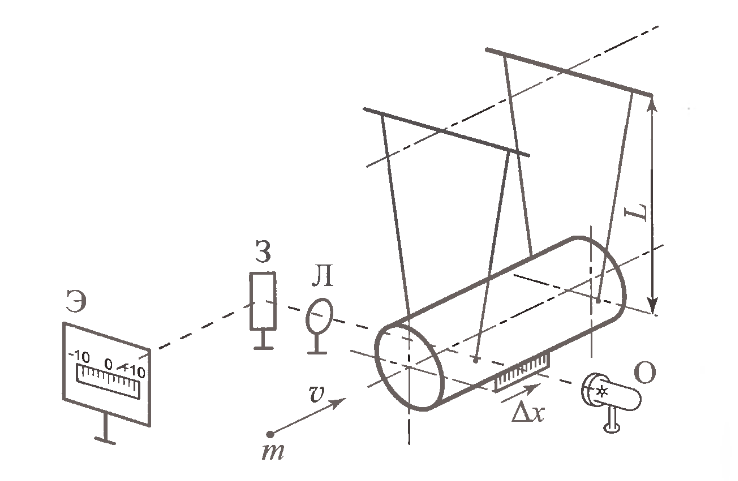
\includegraphics[width=0.9\linewidth]{1.png} 
			\caption{Pис. 1. Схема установки для измерения скорости полета пули}
			\label{fig:subim1}
		\end{subfigure}
		\begin{subfigure}{0.5\textwidth}
			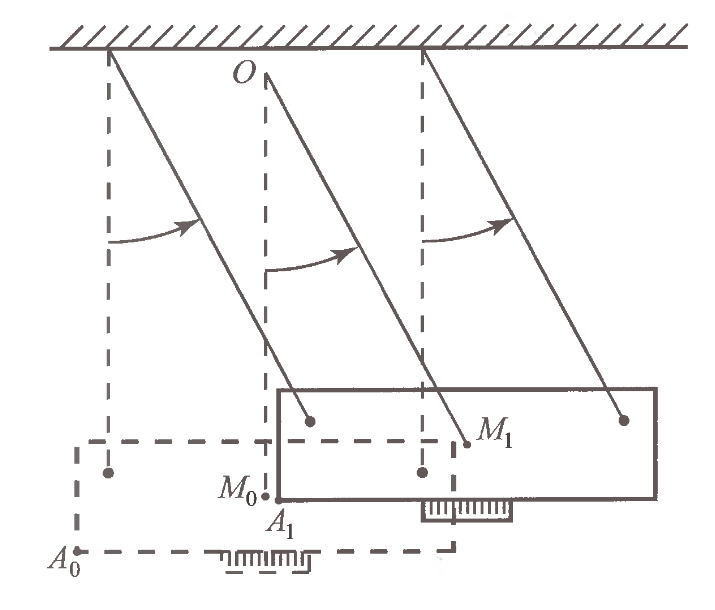
\includegraphics[width=0.9\linewidth]{2.png}
			\caption{Рис 2. Поведение баллистического маятника при попадании в него пули}
			\label{fig:subim2}
		\end{subfigure}
		
	\end{figure}
	
	
	\section{Методика измерений}
	
	\section{Оборудование и инструментальные погрешности}
	\textbf{Оборудование:} духовое ружье на штативе, осветитель, оптическая система для измерения отклонений маятника, измерительная линейка, пули и весы для их взвенивания, а также баллистические маятники.
	
	
	
	\section{Результаты измерений и обработка данных}
	\subsection{Массы пулек:}
	
	$L = (2208\pm10)$ мм, $M=(2900\pm5)$ г.
	
	\subsection{Амплитуды и соответствующие скорости:}
	
	Усредняя, получаем $<v>=(146\pm3)\text{, м/c}$.
	\section{Обсуждение результатов}
	
	\section{Заключение}
	
\end{document}
